\chapter{Bioethics: Designer Children}

These notes follow Michael Sandel's thirteenth \emph{Justice} lecture at CCCB, in the LazyLearn track curated by LazyingArt LLC with Video2Book. The lecture proceeds by a chain of carefully staged boundary questions: first a hard case about deafness, then a widening inquiry into the meaning of health, then a diagnosis of how reproductive choice becomes consumer choice, and finally a political question about who will decide the limits of biotechnology. The formal structure is conceptual rather than quantitative, but the lecture still has a definite mathematical spine: forks, implication chains, and a closing institutional bifurcation.

\section{The Opening Case: A Deaf Couple and a Deaf Child}

Sandel begins with a story rather than with a principle. A lesbian couple wanted a child; they wanted the child to be born deaf; and because both partners were themselves deaf, they sought out a sperm donor who was also deaf and who had five generations of deafness in his family. They conceived a child, and the child was born deaf. The point of the opening is not heredity in the scientific sense. It is intentionality. The trait at issue is not merely suffered or inherited by chance; it is selected for.

The lecture's opening broadcast graphic is worth keeping because it fixes the order of the case without pretending to explain it. It gives us a couple, a donor, and a child, arranged from left to right, and it marks the adults and the infant with the same small head-adjacent sign.

\begin{figure}[h]
\centering

\includegraphics[width=0.62\textwidth]{lecture_13_figure_02.png}
\end{figure}

What the image gives us, and no more, is the visible sequence
\begin{equation}
\text{couple}
\qquad
\text{donor}
\qquad
\text{child}.
\end{equation}
It contains no written genetics, no arrows, and no labels. That is precisely why it is useful: it keeps before us the lecture's initial structure without over-formalizing what the screen does not show.

A cleaned redraw can therefore remain minimal and schematic:

\begin{figure}[h]
\centering
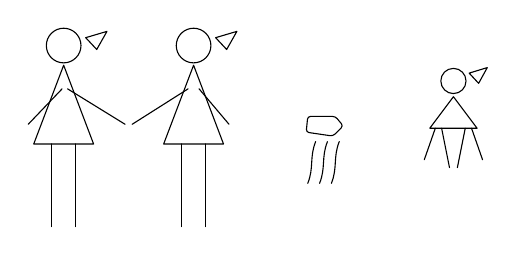
\begin{tikzpicture}[x=1cm,y=1cm,line cap=round,line join=round]
\draw (0,3.0) circle (0.22);
\draw (0,2.75)--(-0.38,1.75)--(0.38,1.75)--cycle;
\draw (-0.15,1.75)--(-0.15,0.7);
\draw (0.15,1.75)--(0.15,0.7);
\draw (-0.02,2.45)--(-0.45,2.0);
\draw (0.05,2.45)--(0.78,2.0);
\draw (0.28,3.10)--(0.55,3.18)--(0.42,2.95)--cycle;

\draw (1.65,3.0) circle (0.22);
\draw (1.65,2.75)--(1.27,1.75)--(2.03,1.75)--cycle;
\draw (1.50,1.75)--(1.50,0.7);
\draw (1.80,1.75)--(1.80,0.7);
\draw (1.58,2.45)--(0.87,2.0);
\draw (1.72,2.45)--(2.10,2.0);
\draw (1.93,3.10)--(2.20,3.18)--(2.07,2.95)--cycle;

\draw[rounded corners=1pt] (3.10,2.10)--(3.45,2.10)--(3.55,1.98)--(3.42,1.85)--(3.08,1.90)--cycle;
\draw (3.20,1.78) .. controls (3.12,1.58) and (3.18,1.45) .. (3.10,1.25);
\draw (3.35,1.78) .. controls (3.27,1.58) and (3.33,1.45) .. (3.25,1.25);
\draw (3.50,1.78) .. controls (3.42,1.58) and (3.48,1.45) .. (3.40,1.25);

\draw (4.95,2.55) circle (0.16);
\draw (4.95,2.35)--(4.65,1.95)--(5.25,1.95)--cycle;
\draw (4.72,1.95)--(4.58,1.55);
\draw (5.18,1.95)--(5.32,1.55);
\draw (4.80,1.95)--(4.90,1.45);
\draw (5.10,1.95)--(5.00,1.45);
\draw (5.15,2.65)--(5.38,2.72)--(5.27,2.52)--cycle;
\end{tikzpicture}
\end{figure}

Sandel then states the philosophical pressure directly. The couple argued that deafness is not a disability but a distinctive identity. That transforms the case at once into a formal fork:
\begin{equation}
\text{deafness}
\stackrel{?}{=}
\text{disability}
\qquad \text{or} \qquad
\text{deafness}
\stackrel{?}{=}
\text{distinctive identity}.
\end{equation}

\subsection{Question \& Answer}

\paragraph{Question.} Is deafness here being treated as a disability imposed on the child, or as a distinctive identity intentionally shared?

\paragraph{Answer.} Sandel does not begin by declaring a winner. His immediate point is methodological: this is exactly the sort of case that forces us to ask what counts as harm, what counts as health, and what kind of human difference biotechnology may permissibly produce or preserve. The lecture therefore opens with a controversy, but it quickly becomes an inquiry into classification.

\section{Borderline Cases and the Meaning of Health}

Having opened with one shocking case, Sandel immediately widens the field. If deafness can be described either as pathology or as identity, then what are we to say about a tendency to obesity, or baldness, or orthodontia? The widening matters because it prevents the deaf-child case from remaining an isolated anomaly. It becomes instead the first member of a broader class of borderline interventions.

The lecture's first fully general question can be written as
\begin{equation}
\text{intervention}
\stackrel{?}{=}
\text{medically necessary}
\qquad \text{or} \qquad
\text{purely preferential}.
\end{equation}
Once the examples are placed side by side, the ordinary distinction between cure and choice no longer does all the work for us. We must decide what health means before we can decide what biotechnology may properly do.

\paragraph{Worked inference.} Sandel's line of thought in this part of the lecture is short and exact:
\begin{align}
\text{borderline cases}
&\Longrightarrow
\text{contested meaning of health},\\
\text{contested meaning of health}
&\Longrightarrow
\text{need for public debate about technological limits}.
\end{align}
And Sandel then states the endpoint explicitly:
\begin{align}
\text{new genetic technology}
&\Longrightarrow
\text{public debate about the meaning of health},\\
\text{public debate about health}
&\Longrightarrow
\text{public debate about the limits of genetic technology}.
\end{align}

\subsection{Question \& Answer}

\paragraph{Question.} When is an intervention medically necessary, and when is it merely preferential?

\paragraph{Answer.} Sandel's answer is that no technical rule settles the matter in advance. Once biotechnology reaches traits at the boundary between disease and variation, societies must argue about the categories themselves. We cannot first define health in a morally neutral way and only then apply it; the application forces the argument over the definition.

\section{Popular Culture and the Logic of Selection}

Only after building this classificatory pressure does Sandel pivot to popular culture. Some of the most penetrating criticisms and worries about biotechnology, he says, have come through novels and film. The move is not ornamental. It prepares the next step by making the logic of selection visible before Sandel returns to actual institutions.

The transcript of the film clip is noisy in detail, but its structure is clear enough. A set of possible children is screened, compared, and selected. Sex can be chosen. The issue is no longer simply whether to have a child, but which child to have. In compact form,
\begin{equation}
\text{screening} + \text{parental preference}
\Longrightarrow
\text{selection among possible children}.
\end{equation}
That is the reason this section appears where it does. Sandel wants us to feel, before he names it outright, the slide from healing to choosing, from accepting a child to selecting among candidates.

The clip therefore serves as a diagnostic lens. It dramatizes a mode of agency that the opening case had already suggested, but in a more recognizably consumer form. Having shown that logic in fiction, Sandel turns back to its real institutional embodiment.

\section{Cryobank, Catalogs, and the Consumer Society}

Sandel's next example is California Cryobank, one of the most successful sperm banks in the world. It is a for-profit company. It sells sperm. It screens donors, accepts only a few, and catalogs donor traits in detail. Sandel's pacing here is crucial: he first lets the market machinery become visible, and only then draws the moral lesson.

\paragraph{Worked market example.} The form of the example can be set out as
\begin{align}
\text{cataloged donor traits}
&=
\text{physical characteristics}
+
\text{ethnic origin}
+
\text{college major}
+\cdots,\\
\text{compensation}
&\leq
\$900 \text{ per month},\\
\text{cataloged donor traits}
+
\text{consumer choice}
&\Longrightarrow
\text{reproductive selection as market behavior}.
\end{align}
The numerical datum matters precisely because it is so mundane. Once traits are screened, arranged, and attached to a price, the transaction acquires the grammar of ordinary commerce. The slogan ``Ivy League sperm'' only sharpens what the structure already shows: the market is not merely facilitating reproduction, it is advertising ranked human attributes.

\subsection{Question \& Answer}

\paragraph{Question.} When does reproductive choice become consumer selection?

\paragraph{Answer.} For Sandel, the shift occurs once reproductive materials are screened, cataloged, advertised, and priced according to desirable traits. At that point the practice ceases to look like medicine aimed at health and begins to look like customization within a consumer market.

Now comes the moral diagnosis. Sandel insists that the company need have no explicit eugenic purpose. It may simply want to make money. But that is enough to generate the danger:
\begin{equation}
\text{children and childbearing}
\Longrightarrow
\text{extension of consumer society}
\Longrightarrow
\text{commodification of children}.
\end{equation}
This point occurs here, not later, because the cryobank example already reveals it. Before the lecture ever reaches the phrase ``designer babies,'' the logic of commodification is already in place.

\section{Designer Babies, Responsibility, and the Parent-Child Relation}

Only after diagnosing the market logic in the cryobank case does Sandel enlarge the horizon to the age of designer babies. A fertility clinic proposes to let parents choose traits such as sex, hair color, eye color, and skin color. The lecture's concern is not simply that there will be more options. It is that the parent-child relation itself is altered once traits become design variables.

The lecture's next formal move is therefore
\begin{equation}
\text{genetic design of children}
\Longrightarrow
\text{explosion of parental responsibility}.
\end{equation}
Why an explosion? Because traits that once appeared as gifts, contingencies, or inheritances become attributable to decision. Sandel then sharpens the consequence:
\begin{equation}
\text{expanded design responsibility}
\Longrightarrow
\text{damage to the parent-child relation}.
\end{equation}
Children may come to hold parents responsible for their height, their appearance, perhaps even their academic performance. A power initially celebrated as freedom becomes a new form of answerability.

A later, briefer example of radical engineering only intensifies the same thought. Once biological characteristics are presented as programmable or designable, the language of production begins to displace the language of begetting and receiving.

\subsection{Question \& Answer}

\paragraph{Question.} Would genetic design deepen parental agency, or corrupt the parent-child relation?

\paragraph{Answer.} Sandel's answer is that the increase in agency comes at the cost of the relation itself. The more traits are chosen, the less the child is received as given and the more the child appears as the output of a parental project. Acceptance gives way to manufacture, and care becomes entangled with design responsibility.

At this point the lecture is ready for its explicit verdict:
\begin{equation}
\text{consumer uses of genetic engineering}
\Longrightarrow
\text{morally impermissible}.
\end{equation}
What matters is the order in which Sandel arrives here. He does not begin with condemnation. He earns it through the opening case, the widening class of borderline interventions, the logic of selection, the cryobank example, and the analysis of parental responsibility.

\section{Market or Democracy: Who Decides the Limits?}

The lecture closes by turning from moral diagnosis to institutional choice. Once the danger has been named, the issue is no longer merely whether commodification is troubling. The issue is who will decide what is to be permitted and what is to be limited. Sandel's closing fork is almost theorem-like:
\begin{equation}
\text{ultimate decision agency}
=
\text{market}
\;\;\text{or}\;\;
\text{democratic institutions}.
\end{equation}
And the more precise conditional is the one on which the lecture ends:
\begin{equation}
\text{no public collective decision}
\Longrightarrow
\text{market decides by default}.
\end{equation}
This is a strong and clarifying end. The alternative is not decision versus indecision. If democratic societies fail to deliberate publicly about the ethical limits of biotechnology, those limits will still be set in practice, only now by the logic of demand, supply, and private purchasing power.

\subsection{Question \& Answer}

\paragraph{Question.} If society does not decide collectively, who decides by default?

\paragraph{Answer.} The market. That is Sandel's final institutional point. The lecture ends not with resignation, but with the claim that democratic institutions must take up the question precisely because markets will otherwise answer it on their own.

\section{Summary}

The lecture unfolds by widening the implications of a single hard case. The deaf-child case forces the opening fork between disability and identity. The rapid list of obesity, baldness, and orthodontia then converts that fork into a broader argument about the meaning of health. Popular culture makes the logic of selection vivid, California Cryobank shows that logic operating in real institutions, and the prospect of designer babies shows how consumer choice can spill over into a transformed parent-child relation.

The final claim is both moral and political. Consumer uses of genetic engineering are, for Sandel, morally impermissible because they threaten to turn children into objects of preference and parenthood into a form of design management. And if democratic societies do not decide collectively where biotechnology should stop, the market will decide for them.